%%%%%%%%%%%%%%%%%%%%%%%%%%%%%%%%%%%%%%%%%%%%%%%%%%
\documentclass[b5paper,11pt, titlepage]{book}
%%%%%%%%%%%%%%%%%%%%%%%%%%%%%%%%%%%%%%%%%%%%%%%%%%
\usepackage[pdftex]{graphicx,color}
%\usepackage[T1,plmath]{polski}
\usepackage[cp1250]{inputenc}
\usepackage{indentfirst}
\usepackage[numbers,sort&compress]{natbib} % sort and compress citations
%\usepackage[none]{hyphenat} % brak podzia�?u wyraz??w
\usepackage{geometry}
\newgeometry{tmargin=3.6cm, bmargin=3.6cm, lmargin=3.2cm, rmargin=3.2cm}
\usepackage{multirow}
\usepackage{amsmath}
\usepackage{adjustbox}
	
\renewcommand{\figurename}{Fig.}
\renewcommand{\tablename}{Tab.}

%%%%%%%%%%%%%%%%%%%%%%%%%%%%%%%%%%%%%%%%%%%%%%%%%%
\begin{document}
%%%%%%%%%%%%%%%%%%%%%%%%%%%%%%%%%%%%%%%%%%%%%%%%%%
%\title{\textbf{Modelowanie struktur anizotropowych \\Wst�pne badania eksperymentalne\\
%	\vspace{10cm}}
%\normalsize{Abstract} }
%\normalsize{W ramach projektu pt.: \\ \textit{Wp�yw jednoczesnego oddzia�ywania temperatury i wilgotno�ci \\na struktury anizotropowe: od teorii do bada� do�wiadczalnych\\}
%NCN OPUS 12}}
	
%{Micha� Jurek}

%\date{ }
	
%\date{Gda�sk, Maj 2018\\ (Nr Arch. 221/2018)}


	
%\maketitle
%\newpage
%\tableofcontents
%\newpage
%\listoffigures
%\listoftables
%\newpage

\chapter{Introduction to Structural Health Monitoring and Artificial Intelligence}
\textbf{Saeed Ullah}
%%%%%%%%%%%%%%%%%%%%%%%%%%%%%%%%%%%%%%%%%%%%%%%%%%
\section{Structural Health Monitoring (SHM)}
%%%%%%%%%%%%%%%%%%%%%%%%%%%%%%%%%%%%%%%%%%%%%%%%%%
Numerous civil engineering and aerospace structures are exceeding or approaching their design lives. Therefore, assessing the condition of these structures is essential in order to determine their serviceability, safety
and load-carry capacity\cite{Chang2000}. It is very crucial to monitor the health of structural elements in mechanical, civil and aerospace industries where the presence of small defects may result in a very catastrophic failure. A defect or damage can be defined as any degradation in the structural parameters which changes the dynamic behavior of the structure\cite{Chang2000}. These changes can be in a micro-scale level such as material matrix anomalies or in the macro-scale level such as cracks. Damage adversely affect the current or future performance of the system. Recently, damage detection methods have been widely studied for the purpose of locating and quantifying structural damages\cite{Chang2000}. There are many ways and indicators for detecting damage in a structure such as variations in strain, natural frequencies, time signal, etc.\cite{DeLuca2020}. Damage detection is usually accomplished in the context of one or more closely related disciplines which include: structural health monitoring (SHM), nondestructive evaluation (NDE) also known as nondestructive testing (NDT), condition monitoring (CM), health and usage monitoring system (HUMS), damage prognosis (DP) and statistical process control (SPC)\cite{Farrar2007, Farrar2012}. SHM can be defined as the process of implementing a damage detection and health assessment strategy for civil, mechanical engineering or aerospace  infrastructure\cite{Farrar2007, Farrar2012}. This process includes continuous monitoring of a mechanical system or structure using dynamic response measurements. For determining the current state of system health, the damage-sensitive features extracted from these measurements are used\cite{Farrar2007, Farrar2012}. The output of these measurements can be periodically updated for long-term SHM. These measurements are very helpful in the case of an extreme event. SHM could be used for providing, in near real time, reliable information and rapid condition screening about the performance of the system\cite{Farrar2012}. SHM aims to detect, identify and characterize the damage and degradation in engineering structures. Sensors are used in the SHM system for monitoring physical quantities such as temperature, acceleration, humidity, tensile and compressive stress, and so on.\cite{Lamonaca2018}. SHM systems' for damage detection needs few special characteristics such as (i) low possibility of missing the damage (ii) rapid calculation (iii) suitability for continuous on-line monitoring (iv) handling of huge information applicable for large engineering structures\cite{lee2008overview}.

SHM systems� tasks can be categorized as a process composed of five activities that form five important levels or elements, as shown in Figure 1.1. These are: (i) damage detection, (ii) damage localization, (iii) damage size assessment, (iv) remaining life prediction, and (v) smart structures with self-evaluating, or control capabilities, also known as life prognosis\cite{stepinski2013advanced,TibaduizaBurgos2020,Scuro2018}. 
\begin{figure} [h!]
	\begin{center}
		\centering
		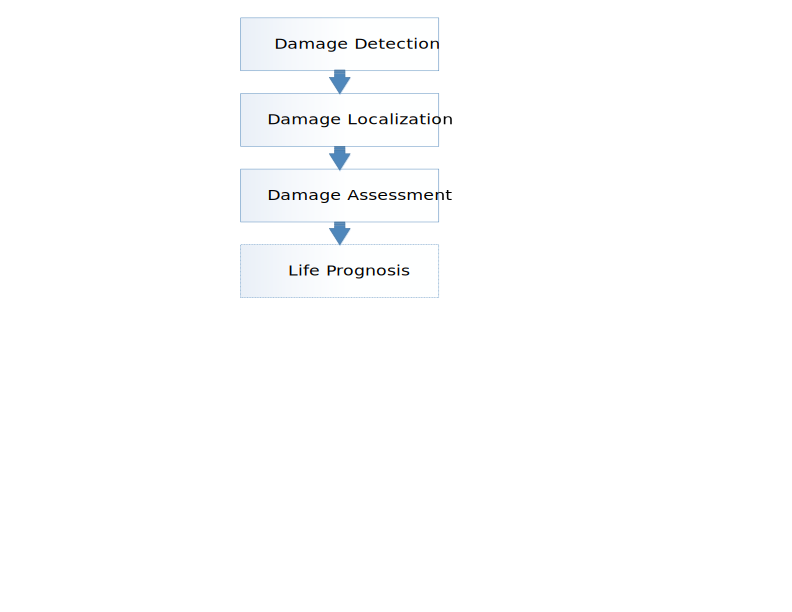
\includegraphics[width=0.7\textwidth]{fig1.1.png}
	\end{center}
	\caption{Five Main levels of SHM Techniques} 
	\label{fig:fig1.1}
\end{figure}

According to these levels, detection gives a qualitative explanation that the damage may exist, localization gives an indication about the probable position of the damage, assessment indicates the estimation of damage severity by giving information about the size and type of damage and at last, the estimation of residual structural life is provided at remaining life and smart structures (prognosis) stage. It also predicts possible failures or breakdowns. The first three levels (i.e. detection, localization, and assessment) are usually related to system identification, signal processing, and modelling aspects. The last two levels fall into statistical analysis, reliability, fatigue analysis, fracture mechanics, and design assessment fields. Many researchers have comprehensively investigated the last two levels but currently, there are no commercially available solutions.\cite{stepinski2013advanced,TibaduizaBurgos2020}. 


\section{SHM and Nondestructive Evaluation/Testing (NDE/T)}
%%%%%%%%%%%%%%%%%%%%%%%%%%%%%%%%%%%%%%%%%%%%%%%%%%
Damage detection or monitoring, NDE/T and SHM are usually mixed up as same things and may have the same meaning in many engineering areas. Health, damage, and monitoring of structures can be interpreted using different definitions. Generally, health is the ability to perform and maintain structural integrity all over the whole lifetime of the structure. However, monitoring is the process of assessment and prognosis, and damage is functional or structural failure in a material\cite{stepinski2013advanced}.

Typically, SHM is identified as online�global damage identification method in
structural systems. Whereas, NDE/T is usually performed as off-line in a local manner once the damage has been located. NDE/T is usually performed periodically for improving the performance of a structure. However, it is not essential as NDE/T is also used as a monitoring tool for in situ structures such as rails and pressure vessels. NDE/T is primarily used for severity check and damage characterization when the damage location is already known\cite{Farrar2007,Farrar2012}.

SHM involves integrating actuators and sensors, possibly smart materials, computational power and data transmission within a structure in order to detect, assess, localize, and predict damage. A typical SHM system is concerned with an online global damage identification in structures; SHM based systems are most often applied in civil engineering and aerospace. SHM systems employ NDE/T methods as tools, however, there are many differences in SHM and NDE/T operation principles\cite{stepinski2013advanced}. 

NDE/T techniques are often bounded to single point measurements. SHM methods allow for online monitoring of large structures and also can perform damage localization. With new sensors, SHM based methods are suitable for reliable continuous monitoring. For reliable damage detection, the SHM needs more state-of-the-art signal processing than classical NDE/T techniques \cite{stepinski2013advanced}.

The main difference between SHM and NDE/T techniques can be observed from the hardware architecture. In an SHM system, actuators and sensors are integrated with or built into the structure, while there is no integration involved with the structures in case of NDE/T. NDE/T is an external system with an independent set of actuators and sensors\cite{stepinski2013advanced}.

Most of the NDE/T techniques need component disassembly particularly for the those components which are inaccessible. The disassembling of components in NDE/T causes disruption of the daily operations. In the process of changing from NDE/T to SHM, cheaper and smaller sensors have been brought. Disassembling is done in SHM only when it is necessary, SHM is helpful in lowering costs as compared to NDE/T. Most of the NDE/T methods are often expensive, labor-intensive and time-consuming. NDE/T techniques highly depend on the experience and skills of the operator. Generally, NDE/T measurements are  qualitative, it is very difficult to verify the reliability of NDE/T measurements. Safety precautions are also essential for most of the NDE/T methods. SHM is primarily focused on condition-based maintenance. Nowadays, SHM is becoming more vital in many engineering fields such as civil, mechanical, and aerospace. SHM is widely adapted by the aerospace community, especially in aging of aircraft situations. SHM is modified and improved version of NDE/T which aims at online or in-service implementation. NDE/T is gradually transferring to a more permanent attachment and constant monitoring, and hence toward SHM.

\section{The Importance of SHM}
%%%%%%%%%%%%%%%%%%%%%%%%%%%%%%%%%%%%%%%%%%%%%%%%%%
Almost all government and private industries are interested in detecting damage in their products and manufacturing structures at the earliest feasible time. These industries carry out some form of SHM for such detection\cite{Farrar2007}. The main aim of the SHM system is to maintain information on the state of the inspected structure for the purpose of finding structural defects before they reach critical levels. It also helps in providing adequate information for condition-based maintenance.

The SHM is an efficient approach for the regular monitoring of roads, bridges, skyscrapers, mechanical, civil, and aerospace structures. The new methods and technological developments are being employed in the SHM. The principal benefits of the employment of SHM include longer life spans, increased safety, detection of early risks and cost-efficiency. Public safety is greatly improved with the use of new SHM methods. Regular monitoring and analysis assist in identifying design flaws. SHM is also helpful in recognizing environmental factors that may not have been taken into consideration during the construction process. Emergency maintenance and a continual preventative of different structures aids to improve their longevity. Another main advantage of SHM is that it greatly reduces short and long-term structural maintenance costs. Furthermore, structural integrity maintenance for a longer span of time lessens overall costs related to rebuilding and demolition\cite{Lamonaca2018}. 

SHM offers an automated inspection process to reduce unessential maintenance tasks. Industries are using SHM as a tool for preventing sudden damage which yields essential benefits to the industries. SHM improves the safety and functionality of structures. SHM is useful in timely warning of impending failures\cite{TibaduizaBurgos2020}.

In an SHM system, data is gathered on realistic performance, which will help to design improved structures for the future. SHM is able to ensure safety and avoid the failure of the structure which in turn will save uncountable human losses due to accidents. In conventional system, a considerable number of structures undergo regular assessment and maintenance for the purpose of ensuring the structural stability of the system. This number can easily be reduced by implementing an SHM system which will indicate the healthy structure to be unnecessary for the inspection.
\section{Classification of SHM Techniques}
%%%%%%%%%%%%%%%%%%%%%%%%%%%%%%%%%%%%%%%%%%%%%%%%%%
Damage detection methods for SHM can be categorized into two main groups based on the type of information to be used: Local and Global methods. 

Local techniques monitor a tiny part of the structure surrounded by sensors using measurements of structural response. Acoustic emission, magnetic fields, radiography, eddy currents, ultrasonic waves, �and thermal field are some examples which are commonly employed for local SHM\cite{lee2008overview, stepinski2013advanced}.
\newline The global methods are executed when global motion is induced in the structure during its operation. Vibration-based methods are one of the examples of this class. Global methods are helpful when local damage has an influence on the behavior of the global structure in terms of space and time. 
As opposed to local methods, global methods have many benefits: 
\newline i) The whole structure can be measured with these methods by using a rough sensor network.
\newline ii) It is not necessary to locate sensors near the damage.
\newline iii) Only a little information about the critical location is enough. 
Global methods also have some disadvantages: 
\newline i) The wavelength of vibrations is nearly equivalent to the dimension of the component or structure, therefore, these methods have relatively low sensitivity to small damages. 
\newline ii) Usually these methods are quite expensive.

Although the damage size and location are roughly estimated with these methods it can successfully be used for damage detection. The relationship between defects of structures and structural vibration is used in the health assessment. Global methods can be further divided into two types of methods: model-based and signal-based. The model-based methods utilize different kinds of models of a monitored structure to localize and detect the defect in the structure. These models use relations between particular damages and model parameters. In these methods, the comparison of damaged and undamaged structures are taken into account for detection and localization of damage. The relation between measured responses of the structures is employed in signal-based methods. Currently, signal features in time, frequency, and time/frequency domains are very popular. These methods are usually applied in diagnostics of reciprocating and rotating machinery for damage detection, but for damage assessment and localization more additional information is also needed\cite{stepinski2013advanced,Worden2007}. 
\section{Basic Elements of SHM}
%%%%%%%%%%%%%%%%%%%%%%%%%%%%%%%%%%%%%%%%%%%%%%%%%%
Mostly, an SHM system is represented as an online global damage identification system in structures. SHM systems are composed of three key elements: (i) A network of actuators and sensors, most likely smart materials, which are permanently attached to the structure. This aspect of SHM makes it different from conventional NDT techniques and it is mandatory for executing automated inspections. This step involves observation of the structure from arrays of sensors using regular sampled response measurements, storing the measured data, and transmitting data to the control center. (ii) On-board information handling and computing facilities. A large number of sensors are continuously producing a huge amount of data to be processed in real-time. Computational power and data transmission are employed within a structure for the purpose of detecting, localizing, assessing and predicting damage which can cause structure impairment now or in the future. (iii) Algorithms that analyze stored data from the structure with recently acquired data. Algorithms calculate a damage index and then inform about damage presence, localization, and type\cite{stepinski2013advanced}. "Cite another paper here..11. Structural Health Monitoring for Advanced Composite Structures A Review"

For monitoring of possible changes in the structures, all SHM systems need a proper sensor network. The sensibility of the SHM system is usually associated with good interaction between the sensors and the structure. Therefore, it is very important to choose the appropriate sensors to be installed. During the implementation of network of sensors in an SHM system, the information for obtaining defect identification, the material of the structure to inspect, the variables to sense or measure are considered. The next stage is data acquisition, also known as DAQ. In this stage, the signals produced by each sensor are obtained. At this stage, the SHM system�s characteristics, such as mobility, cost, scalability need to be considered. The information collected by the SHM system can be affected by sensor configuration, environmental and operational noise, or any other event. Many of these problems must be resolved before executing any analysis on the produced information for generalizing the techniques used for recognition, identification or classification. This step is associated with preprocessing or signal conditioning. It can be performed with the use of hardware devices, software algorithms, or both. At last, data analysis tools are used for determining the existence of damage in the instrumented structure and for characterizing the possible source of the damage\cite{TibaduizaBurgos2020}. "Cite another paper here.12. Introduction to Structural Health Monitoring".
\section{Types of Sensors used in SHM}
%%%%%%%%%%%%%%%%%%%%%%%%%%%%%%%%%%%%%%%%%%%%%%%%%%
In last few years, structural engineering community are increasingly implementing sensor networks for SHM purposes of monitoring structures. For an SHM system, it is essential to acquire proper assessment of a system�s dynamic response. There are several different types of sensors and data acquisition systems that can be applied to the SHM problem. The sensors employed in an SHM system are application specific\cite{Farrar2012}.

SHM sensing system consist of some or all of the following components:
\newline 1. Transducers that are responsible for converting changes in the field variable of interest i.e. temperature, strain, or acceleration to changes in an electrical signal i.e. resistance, voltage, or impedance.
\newline 2. Actuators that are responsible for applying a recommended input to the system i.e. a piezoelectric transducer attached to the surface of a structure.
\newline 3. Analogue-to-Digital (A/D) converters that are responsible for converting analogue electrical signal into a digital signal that can be processed on digital hardware. Those SHM systems which are using actuators, a Digital-to-Analogue (D/A) converter is also needed for converting a prescribed digital excitation signal to an analogue voltage which is useful for controlling the actuator\cite{Farrar2012}. 

Damage detection for an SHM needs the employment of a set of sensors with the main function of capturing information which can be used for determining the state of the structure under inspection. Many SHM systems use the propagation of a signal that is produced by an actuator. The inspection also depends on the transducer type used for inspection and the kinds of propagated signals over the structure. The transducers employed in SHM system should be light and small in size for the purpose of integration into the structure without any considerable impact on its behavior. With the increased implementation of SHM approaches, new sensors have been developed. These new sensors are very helpful in improving the ability of detection, characterization, and localization of defects in an SHM system. These advancements in sensors aim to reduce the weight and power consumption of the system. In addition, it also helps in resolving installation problems, and for improving operation facilities and subsequent data analysis. The following subsections illustrate some of the different types of sensors used in SHM systems. These sensors can be adapted for the inspection of both composite and metallic structures. A rightly chosen sensor not only detect defects but also enables SHM system to correctly perform damage location, quantification, and classification. Sensors can be categorized on the basis of physical variable which they sense or on the principle of transduction on which they are based. Some of these sensors, their advantages, disadvantages and the inspected variable is shown in Table 1.1\cite{Farrar2012,TibaduizaBurgos2020}.

\subsection{Piezoelectric Sensors:}
Piezoelectric materials are built from polymers and ceramic. Piezoelectric transducers are a category of device that satisfy most of the demands of SHM. PZT transducers are light weight, small in size, consume a low amount of power, and are able to generate frequency response in a wider region. PZT transducers are less expensive and their size is relatively small in comparison to the size of the monitored structures. Some other advantages of piezoelectric sensors are: these sensors can be assembled in various shapes, such as longitudinal, rectangular, and circular. These sensors are also very flexible and can easily be fitted to the shape of the structure at their installation regions. These transducers can be used for rapid and in situ SHM. PZT transducers can easily be arranged as a network of sensors in order to record multipoint measurements on or under the surface of the monitored structure. However, the methods utilizing these transducers mostly needs a large number of data points and the baseline signal for the purpose of comparison with the damaged signal for authentic damage estimation.
"The Above text is taken \cite{Farrar2012} and 15.  Lamb-Wave-Based Multistage Damage Detection Method Using an Active PZT Sensor Network for Large Structures."
PZT based transducers are mostly used for sensing and generation of guided waves. With PZT based transducers, it is easy to measure the vibration and acquire information about different variables, such as corrosion or deformation. 
\newline "The Above text is taken from \cite{TibaduizaBurgos2020} and from 14. Guided wave based structural health monitoring A Review."

Arranging piezoelectric sensors for inspecting composite materials are described as piezoelectric inspection. Piezoelectric inspection can be considered as one of the active research areas of SHM based techniques. This technique uses a network of PZT transducers embedded into or attached onto the host composite.
\newline "The above text is taken from 13. A Survey of Scrutinizing Delaminated Composites."
\subsection{Fiber Optics:}
Fiber optics are employed in those applications where high precision and electromagnetic-interference freedom is required. The principle underlying these sensors are based on white-light intervention, which can relate the complete shifting of a signal radiated from a light source with any physical variable. This type of sensors is useful for measuring temperature, acceleration, vibrations, pressure, rotation, deformation, material concentrations, and shifting. For deformation measurements, Fiber Optics Sensors (FOS) and Fiber Bragg Grating (FBG) sensors are mostly used. FOS are less costly, usually contains multimode fibers, and auto-compensate for temperature changes. Whereas, FBG sensors are used as selective filters of any wavelength\cite{TibaduizaBurgos2020}. 
\subsection{Microelectromechanical Systems (MEMS):}
Miniaturization techniques are used in the construction of this type of sensors and it combines different types of transducers. These sensors are very beneficial in case of the costs of maintenance and implementation. These type of sensors have some other attractive features too, such as their small size or their ability of easily connectivity with a wireless sensor network. It is even possible to find sensors that use inductive, capacitive, optical effects or piezoelectric. In addition, actuators can also be included. Generally, MEMS are composed of the integration of various types of sensors. MEMS are used for measuring the magnitude of diverse variables, such as angular velocity (gyroscopes), displacement, acceleration and deformation. This type of sensor provides high sensitivity, the integration of communication systems, responses at low frequencies, and the measurement of multiple variables. Recently, the use of MEMS sensors has significantly increased due to the mentioned factors\cite{TibaduizaBurgos2020}.
\begin{table}[h]
	\centering
	\caption{Types of Sensors Used in SHM}
    \begin{adjustbox}{width=\textwidth}
	\begin{tabular}{|c|c|c|c|c|}
		\hline
		Sensor Type                                                                                                            & Technology                   & Variable to Measure                         & Advantages                                                                           & Disadvantages                                                     \\ \hline
		\multirow{5}{*}{Piezoelectric}                                                                                         & PZT                          & Acceleration                                & Low Cost                                                                             & Thermal Sensitivity                                               \\ \cline{2-5} 
		& PVDF                         & Deformation                                 & Low Price                                                                            & Aging                                                             \\ \cline{2-5} 
		& \multirow{3}{*}{P(VDF-TrFE)} & Corrosion                                   & Integration Possibilities                                                            &                                                                   \\ \cline{3-5} 
		&                              & Vibration                                   & \multicolumn{1}{l|}{}                                                                & \multicolumn{1}{l|}{}                                             \\ \cline{3-5} 
		&                              & Displacement                                & \multicolumn{1}{l|}{}                                                                & \multicolumn{1}{l|}{}                                             \\ \hline
		\multirow{6}{*}{Fiber Optics}                                                                                          & \multirow{5}{*}{FOS}         & Rotation                                    & \begin{tabular}[c]{@{}c@{}}Electromagnetic Interference\\  Immunity\end{tabular}     &                                                                   \\ \cline{3-5} 
		&                              & Acceleration                                &                                                                                      & Fragility                                                         \\ \cline{3-5} 
		&                              & Vibrations                                  & Integration Possibilities                                                            & \multicolumn{1}{l|}{}                                             \\ \cline{3-5} 
		&                              & Pressure                                    & \multicolumn{1}{l|}{}                                                                & \multicolumn{1}{l|}{}                                             \\ \cline{3-5} 
		&                              & Shifting                                    & \multicolumn{1}{l|}{}                                                                & \multicolumn{1}{l|}{}                                             \\ \cline{2-5} 
		& FBG                          & Deformation                                 & High precision                                                                       & High price                                                        \\ \hline
		\multicolumn{1}{|l|}{\multirow{5}{*}{\begin{tabular}[c]{@{}l@{}}Microelectromechanical\\ Systems (MEMS)\end{tabular}}} & MEMS                         & Deformation                                 & Low cost                                                                             & \begin{tabular}[c]{@{}c@{}}High-frequency\\ Response\end{tabular} \\ \cline{2-5} 
		\multicolumn{1}{|l|}{}                                                                                                 & \multirow{4}{*}{NEMS}        & Deformation                                 & \begin{tabular}[c]{@{}c@{}}Different Kinds of\\ Sensors and\\ Variables\end{tabular} & \multicolumn{1}{l|}{}                                             \\ \cline{3-5} 
		\multicolumn{1}{|l|}{}                                                                                                 &                              & Displacement                                & Wireless Connection                                                                  & \multicolumn{1}{l|}{}                                             \\ \cline{3-5} 
		\multicolumn{1}{|l|}{}                                                                                                 &                              & \multicolumn{1}{l|}{Acceleration Gyrometer} & Small Size                                                                           & Fragility                                                         \\ \cline{3-5} 
		\multicolumn{1}{|l|}{}                                                                                                 &                              & Shifting                                    & \multicolumn{1}{l|}{}                                                                & \multicolumn{1}{l|}{}                                             \\ \hline
	\end{tabular}
	\end{adjustbox}
\end{table}
\section{Guided Waves Based SHM}
%%%%%%%%%%%%%%%%%%%%%%%%%%%%%%%%%%%%%%%%%%%%%%%%%%
text
\section{SHM in Composite Structures}
%%%%%%%%%%%%%%%%%%%%%%%%%%%%%%%%%%%%%%%%%%%%%%%%%%
text
\section{Major Challenges in SHM}
%%%%%%%%%%%%%%%%%%%%%%%%%%%%%%%%%%%%%%%%%%%%%%%%%%
text
\section{Artificial Intelligence, Machine Learning and Deep Learning}
%%%%%%%%%%%%%%%%%%%%%%%%%%%%%%%%%%%%%%%%%%%%%%%%%%
text
\section{AI, ML and DL in SHM}
%%%%%%%%%%%%%%%%%%%%%%%%%%%%%%%%%%%%%%%%%%%%%%%%%%
text
%%%%%%%%%%%%%%%%%%%%%%%%%%%%%%%%%%%%%%%%%%%%%%%%%%
%\subsection{Description}
%%%%%%%%%%%%%%%%%%%%%%%%%%%%%%%%%%%%%%%%%%%%%%%%%%
%text
%%%%%%%%%%%%%%%%%%%%%%%%%%%%%%%%%%%%%%%%%%%%%%%%%%

%\begin{figure} [h!]
%	\begin{center}
		%\includegraphics[width=14cm]{Graphics/bc.jpg}
%	\end{center}
%	\caption{Figure caption.} 
%	\label{fig:bc}
%\end{figure}

%%%%%%%%%%%%%%%%%%%%%%%%%%%%%%%%%%%%%%%%%%%%%%%%%%

%\begin{table}[h]
%\centering
%	\caption{Table caption}
%	\begin{tabular}{cccc}
%		\hline
%	\textbf{a}	& \textbf{x} & \textbf{y} & \textbf{z} \\
%		\hline
%		-50 & -0.289 & -0.289 & -0.598\\ 
%		-40 & -0.248 & -0.248 & -0.512\\ 
%		\hline 
%	\end{tabular} 
%	\label{tab:xyz}
%\end{table}
%%%%%%%%%%%%%%%%%%%%%%%%%%%%%%%%%%%%%%%%%%%%%%%%%%

%The scheme of experimental setup is shown in Fig.~\ref{fig:bc}.  
%The values are collected in Tab.~\ref{tab:xyz}.


%The details are described in a book~\cite{udd2011fiber}. 

%Similar case was analysed\cite{Badrinarayanan2017a} by Hill et al.
%Additional information:
%\begin{itemize}
%\item fonts Times New Roman, 11pt
%\item keep figures separately in greyscale with resolution 600 dpi (publisher requirement)
%\item 20-30 pages
%\item Bibliography\cite references in the order of citations within the text
%\end{itemize}

\bibliography{report} % 
%bibliography data in report.bib
\bibliographystyle{abbrv}
% makes bibtex use spiebib.bst


%%%%%%%%%%%%%%%%%%%%%%%%%%%%%%%%%%%%%%%%%%%%%%%%%%
\end{document}
%%%%%%%%%%%%%%%%%%%%%%%%%%%%%%%%%%%%%%%%%%%%%%%%%%
